\chapter{El problema: dos sensores, dos formas de contar}\label{cap:problema}

\section{La diferencia es de instrumento, no de fuego}

Si sumamos todos los hotspots filtrados de 2013 a 2025, VIIRS cuenta \razonVM{} veces lo que cuenta MODIS en México. Una razón tan grande no puede venir de que haya más fuego en la zona que ve VIIRS, porque ambos sensores observan el mismo territorio. Viene de tres diferencias de instrumento:

\begin{enumerate}[label=\arabic*)]
  \item \textbf{Resolución espacial}: 375 m contra 1 km. Un fuego pequeño que no alcanza a calentar un píxel de 1 km puede encender uno de 375 m.
  \item \textbf{Hora de paso} del satélite sobre cada lugar, que cambia el estado del fuego observado y la cantidad de nubes y de humo.
  \item \textbf{Algoritmo de detección}, con umbrales distintos.
\end{enumerate}

Si pegáramos las dos series tal cual, la serie «saltaría» cuatro veces hacia arriba en 2012 y parecería que las quemas se cuadruplicaron. No es cierto: cambió el instrumento.

\begin{figure}[H]
\centering
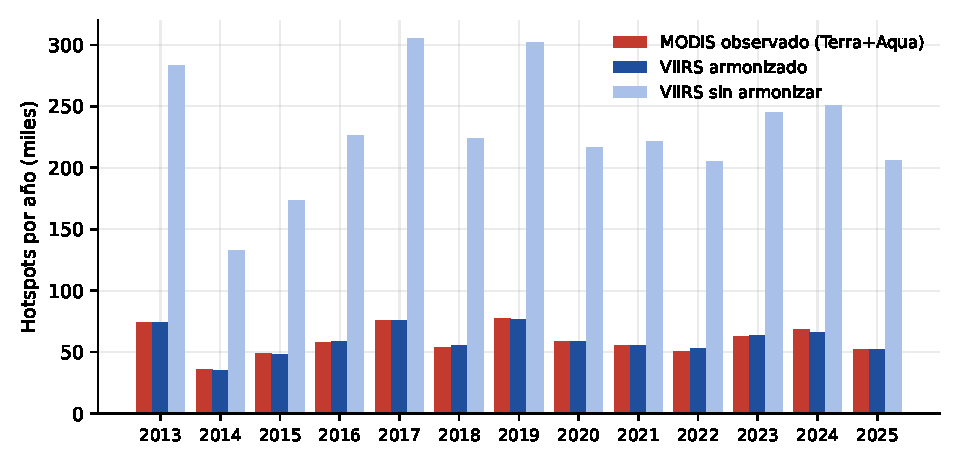
\includegraphics[width=0.95\textwidth]{fig/fig_anual.pdf}
\caption{Hotspots anuales en México, 2013--2025. La barra clara (VIIRS sin armonizar) queda casi cuatro veces por encima de MODIS. Después de armonizar, la barra azul prácticamente coincide con la roja. El factor se calibró con 2012--2019, de modo que el ajuste de 2020 en adelante es fuera de muestra.}\label{fig:anual}
\end{figure}

\section{Qué significa «armonizar»}

La figura~\ref{fig:anual} ya anticipa el objetivo. Queremos asignar a cada detección $i$ de VIIRS un peso $w_i\geq0$ tal que, en cualquier región y mes, la suma de pesos reproduzca \emph{en promedio} lo que habría contado MODIS. Con la notación del capítulo~\ref{cap:datos}, si $H_{y,m,s}=\sum_{i\in(y,m,s)} w_i$ es la suma de pesos,
\begin{align*}
  \E\!\left[H_{y,m,s}\right] &= \E\!\left[M_{y,m,s}\right].
\end{align*}
Esta es la propiedad que queremos y, además, la que verificamos con datos que el método no vio (capítulo~\ref{cap:valid}).

\begin{definicion}[Unidad común: el hotspot equivalente a MODIS]
Un \emph{hotspot equivalente a MODIS} es lo que habrían contado Terra y Aqua juntos. Una detección de VIIRS vale $k<1$ hotspots equivalentes, porque VIIRS cuenta más que MODIS. Una detección de MODIS posterior a julio de 2002 vale 1 hasta que empieza VIIRS (sección~\ref{sec:etapas}).
\end{definicion}

\section{Por qué el factor depende del estado y del mes}

Si la razón entre lo que cuentan los dos sensores fuera la misma siempre y en todas partes, bastaría un número único. No lo es, porque la razón depende de cuántos fuegos pequeños hay (que cambia con el tipo de vegetación y con la temporada) y de las nubes y del humo (que cambian con la estación). La figura~\ref{fig:knat} muestra que, incluso a escala nacional, la razón de MODIS entre VIIRS pasa de $0.19$ en junio a $0.31$ en diciembre. El capítulo~\ref{cap:result} cuantifica cuánto mejora el resultado al permitir esa variación.

\begin{figure}[H]
\centering
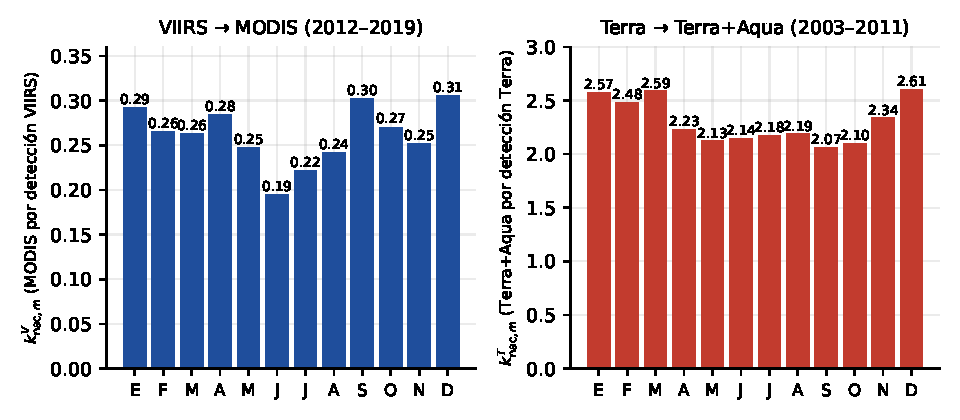
\includegraphics[width=0.98\textwidth]{fig/fig_knat.pdf}
\caption{Factor nacional por mes. Izquierda: hotspots de MODIS por cada detección de VIIRS (calibración 2012--2019). Derecha: hotspots de Terra más Aqua por cada detección de Terra (calibración 2003--2011).}\label{fig:knat}
\end{figure}

\begin{ideaclave}[Idea clave del capítulo]
VIIRS cuenta \razonVM{} veces más que MODIS por razones de instrumento. Armonizar consiste en dar a cada detección de VIIRS un peso $k$ menor que 1, de modo que la suma de pesos reproduzca lo que habría contado MODIS. El peso varía con el estado y con el mes del año.
\end{ideaclave}
